\documentclass[12pt,a4paper]{article}

% ─── Page Layout ───────────────────────────────────────────────────────────────
\usepackage[a4paper, margin=0.8in, headheight=14pt]{geometry}

% ─── Fonts (XeLaTeX) ───────────────────────────────────────────────────────────
\usepackage{fontspec}
\usepackage{unicode-math}
\setmainfont{TeX Gyre Pagella}
\setmonofont[Scale=0.88]{TeX Gyre Cursor}
\setmathfont{Latin Modern Math}

% ─── Packages ──────────────────────────────────────────────────────────────────
\usepackage{xcolor}
\usepackage{colortbl}
\usepackage{titlesec}
\usepackage{enumitem}
\usepackage{tabularx}
\usepackage{booktabs}
\usepackage{array}
\usepackage{amsmath}
\usepackage{tikz}
\usetikzlibrary{shapes.geometric, arrows.meta, positioning, calc, fit, decorations.pathreplacing, patterns}
\usepackage[american]{circuitikz}
\usepackage{tcolorbox}
\tcbuselibrary{skins, breakable}
\usepackage{hyperref}
\usepackage{fancyhdr}
\usepackage{graphicx}
\usepackage{microtype}
\hyphenpenalty=10000
\exhyphenpenalty=10000
\sloppy
\usepackage{caption}
\usepackage{setspace}
\usepackage{multirow}
\usepackage{tocloft}

% ─── Q&A helper ────────────────────────────────────────────────────────────────
\newcommand{\Q}[1]{\textbf{#1}\par\noindent\ignorespaces}

% ─── Colour Palette ────────────────────────────────────────────────────────────
\definecolor{myred}{RGB}{196,30,58}
\definecolor{mydark}{RGB}{30,30,50}
\definecolor{mygreen}{RGB}{14,120,80}
\definecolor{myteal}{RGB}{0,130,140}
\definecolor{myamber}{RGB}{180,100,0}
\definecolor{mypurple}{RGB}{100,30,160}
\definecolor{mygray}{RGB}{246,247,249}
\definecolor{mgframe}{RGB}{180,185,200}
\definecolor{watermark}{RGB}{145,150,170}
\definecolor{hdrred}{RGB}{250,232,235}
\definecolor{hdrgreen}{RGB}{220,244,233}
\definecolor{hdrteal}{RGB}{220,242,244}
\definecolor{hdramber}{RGB}{253,242,215}
\definecolor{hdrpurple}{RGB}{238,228,255}
\definecolor{hdrgray}{RGB}{238,240,245}
\definecolor{rowalt}{RGB}{250,251,253}

% ─── Section Formatting ────────────────────────────────────────────────────────
\titleformat{\section}{\large\bfseries\color{myred}}{\thesection.}{0.5em}{}[\vspace{1pt}{\color{myred}\rule{\linewidth}{0.8pt}}]
\titleformat{\subsection}{\normalsize\bfseries\color{myteal}}{\thesubsection}{0.5em}{}
\titlespacing*{\section}{0pt}{18pt}{7pt}
\titlespacing*{\subsection}{0pt}{11pt}{4pt}

% ─── Paragraph ─────────────────────────────────────────────────────────────────
\setlength{\parindent}{0pt}
\setlength{\parskip}{4pt}

% ─── TOC Styling ───────────────────────────────────────────────────────────────
\renewcommand{\cfttoctitlefont}{\large\bfseries\color{myred}}
\renewcommand{\cftaftertoctitle}{\par\noindent{\color{myred}\rule{\linewidth}{0.8pt}}}
\setlength{\cftbeforetoctitleskip}{0pt}
\setlength{\cftaftertoctitleskip}{6pt}
\renewcommand{\cftsecfont}{\normalsize\bfseries\color{mydark}}
\renewcommand{\cftsecpagefont}{\normalsize\bfseries\color{mydark}}
\renewcommand{\cftsecleader}{\cftdotfill{\cftdotsep}}
\setlength{\cftbeforesecskip}{7pt}
\renewcommand{\cftsubsecfont}{\small\color{mydark}}
\renewcommand{\cftsubsecpagefont}{\small\color{mydark}}
\setlength{\cftbeforesubsecskip}{3pt}
\setlength{\cftsubsecindent}{1.4em}

% ─── Table helpers ─────────────────────────────────────────────────────────────
\renewcommand{\arraystretch}{1.45}
\setlength{\tabcolsep}{6pt}
\arrayrulecolor{mydark}
\newcolumntype{B}[1]{>{\small\bfseries\raggedright\arraybackslash}m{#1}}
\newcolumntype{Y}{>{\small\raggedright\arraybackslash}X}
\renewcommand{\tabularxcolumn}[1]{m{#1}}

% ─── Header / Footer ───────────────────────────────────────────────────────────
\pagestyle{fancy}
\fancyhf{}
\fancyhead[L]{\small\color{myred}\textbf{PE-EC802A}\;\color{mydark}--- Mixed Signal Design}
\fancyhead[R]{\small\color{myteal}\textbf{Module 3 Notes}}
\fancyfoot[C]{\small\color{mydark}\thepage}
\fancyfoot[R]{\small\color{watermark}\textit{\copyright\ Biraj}}
\renewcommand{\headrulewidth}{0.5pt}
\renewcommand{\footrulewidth}{0.3pt}

% ─── Hyperref ──────────────────────────────────────────────────────────────────
\hypersetup{colorlinks=true, linkcolor=myteal, urlcolor=myteal,
  pdfauthor={Biraj Sarkar}, pdftitle={PE-EC802A --- Module 3 Notes}}

% ─── tcolorbox styles ──────────────────────────────────────────────────────────
\tcbset{
  tikzbox/.style={colback=mygray, colframe=mgframe, boxrule=0.6pt, arc=4pt,
    left=8pt, right=8pt, top=6pt, bottom=6pt,
    colbacktitle=mgframe, coltitle=mydark, fonttitle=\small\bfseries},
  defbox/.style={colback=hdrgreen, colframe=mygreen, boxrule=0.8pt, arc=4pt,
    left=9pt, right=9pt, top=6pt, bottom=6pt,
    colbacktitle=mygreen, coltitle=white, fonttitle=\small\bfseries},
  formulabox/.style={colback=hdrteal, colframe=myteal, boxrule=0.8pt, arc=4pt,
    left=9pt, right=9pt, top=7pt, bottom=7pt,
    colbacktitle=myteal, coltitle=white, fonttitle=\small\bfseries},
  examplebox/.style={colback=hdramber, colframe=myamber, boxrule=0.8pt, arc=4pt,
    left=9pt, right=9pt, top=6pt, bottom=6pt,
    colbacktitle=myamber, coltitle=white, fonttitle=\small\bfseries},
  masonbox/.style={colback=hdrpurple, colframe=mypurple, boxrule=0.8pt, arc=4pt,
    left=9pt, right=9pt, top=6pt, bottom=6pt,
    colbacktitle=mypurple, coltitle=white, fonttitle=\small\bfseries},
  exambox/.style={colback=hdrpurple, colframe=mypurple, boxrule=1pt, arc=5pt,
    left=10pt, right=10pt, top=8pt, bottom=8pt,
    colbacktitle=mypurple, coltitle=white, fonttitle=\bfseries,
    breakable, title after break={\textbf{Frequently Asked / Viva Questions (contd.)}}}
}
\tcbset{breakable}

% ─── TikZ styles ───────────────────────────────────────────────────────────────
\tikzset{
  block/.style={rectangle, draw=myteal, fill=hdrteal,
    text width=2.4cm, align=center, minimum height=0.95cm,
    font=\small, rounded corners=3pt, line width=0.7pt},
  redblock/.style={rectangle, draw=myred, fill=hdrred,
    text width=2.4cm, align=center, minimum height=0.95cm,
    font=\small, rounded corners=3pt, line width=0.7pt},
  sumjunc/.style={circle, draw=myamber, fill=hdramber,
    minimum size=0.62cm, font=\small, line width=0.8pt},
  arrow/.style={-Stealth, thick, color=mydark},
  line/.style={thick, color=mydark}
}

% ═══════════════════════════════════════════════════════════════════════════════
\begin{document}
% ═══════════════════════════════════════════════════════════════════════════════

\begin{center}
  {\LARGE\bfseries\color{myred} PE-EC802A --- Mixed Signal Design}\\[5pt]
  {\normalsize\color{mydark} Semester VIII \quad$\bullet$\quad 3L:0T:0P \quad$\bullet$\quad 3 Credits}\\[3pt]
  {\normalsize\color{myteal}\textbf{Module 3 Exam Notes}}\\[3pt]
  {\small\color{mydark} CGEC \;$|$\; B.Tech ECE (2023--27) \;$|$\; \textit{Biraj Sarkar}}
\end{center}
\vspace{2pt}
\noindent{\color{myred}\rule{\linewidth}{1.5pt}}
\vspace{2pt}

\hypersetup{linkcolor=mydark}
\tableofcontents
\hypersetup{linkcolor=myteal}
\newpage

% ===============================================================================
\section{Data Converter Performance Metrics}
% ===============================================================================

Data converters form the bridge between the analog physical world and the digital processing domain. Their performance is specified by static and dynamic parameters.

\subsection{Static Metrics: DNL and INL}
Let $\Delta$ (or $1\,\text{LSB} = V_{FS}/2^N$) represent the ideal step size of the converter.

\begin{tcolorbox}[defbox, title={\textbf{Differential Non-Linearity (DNL)}}]
\textbf{Differential Non-Linearity (DNL)} measures the deviation of an actual step width from the ideal value of $1\,\text{LSB}$. For an ADC, it is the difference between the actual step width $W_k$ and the ideal $1\,\text{LSB}$:
\[
\text{DNL}_k = \frac{W_k - \text{LSB}}{\text{LSB}}
\]
If DNL becomes less than $-1\,\text{LSB}$, the step width becomes zero or negative, leading to \textbf{missing codes} in ADCs. A system is guaranteed monotonic if $\text{DNL} > -1\,\text{LSB}$.
\end{tcolorbox}

\begin{tcolorbox}[defbox, title={\textbf{Integral Non-Linearity (INL)}}]
\textbf{Integral Non-Linearity (INL)} measures the deviation of the actual transfer function characteristics from the straight line (ideal transfer curve) connecting the endpoints (zero-scale and full-scale). It represents the cumulative sum of DNL errors:
\[
\text{INL}_k = \sum_{i=1}^{k} \text{DNL}_i
\]
INL directly limits the harmonic distortion and linearity of the system.
\end{tcolorbox}

\subsection{Quantization Noise Derivation}
Quantization is the process of mapping a continuous range of values to a discrete set. The difference between the continuous input $x$ and its quantized representation $q(x)$ is the quantization error $e = x - q(x)$.

Assuming the input is active and spans many levels, the quantization error $e$ is uniformly distributed between $-\Delta/2$ and $+\Delta/2$. The probability density function (PDF) is:
\[
p(e) = \frac{1}{\Delta} \qquad \text{for } -\frac{\Delta}{2} \le e \le \frac{\Delta}{2}
\]

\textbf{Step-by-Step Derivation of Quantization Noise Power ($v_{qn}^2$):}
\begin{enumerate}[label=\textbf{\arabic*.}, leftmargin=*, itemsep=3.5pt]
  \item The noise power (variance of the error) is:
  \[
  P_{qn} = \sigma_e^2 = \int_{-\Delta/2}^{\Delta/2} e^2 p(e) de = \int_{-\Delta/2}^{\Delta/2} e^2 \frac{1}{\Delta} de
  \]
  \item Evaluating the integral:
  \[
  P_{qn} = \frac{1}{\Delta} \left[ \frac{e^3}{3} \right]_{-\Delta/2}^{\Delta/2} = \frac{1}{3\Delta} \left( \frac{\Delta^3}{8} - \left(-\frac{\Delta^3}{8}\right) \right) = \frac{1}{3\Delta} \left( \frac{2\Delta^3}{8} \right) = \frac{\Delta^2}{12}
  \]
  \begin{tcolorbox}[formulabox, title={\textbf{Quantization Noise Power}}]
  \[
  P_{qn} = \frac{\Delta^2}{12}
  \]
  \end{tcolorbox}
  \item For a sinusoidal input signal of peak amplitude $V_p = V_{FS}/2 = 2^N \Delta/2$, its signal power is:
  \[
  P_{sig} = \frac{V_p^2}{2} = \frac{2^{2N} \Delta^2}{8}
  \]
  \item The Signal-to-Quantization-Noise Ratio (SQNR) is:
  \[
  \text{SQNR} = \frac{P_{sig}}{P_{qn}} = \frac{2^{2N} \Delta^2 / 8}{\Delta^2 / 12} = \frac{12}{8} 2^{2N} = 1.5 \times 2^{2N}
  \]
  \item In decibels (dB):
  \begin{tcolorbox}[formulabox, title={\textbf{Ideal SQNR Equation}}]
  \[
  \text{SQNR (dB)} = 10 \log_{10}(1.5) + 20 N \log_{10}(2) = 1.76 + 6.02 N
  \]
  where $N$ is the resolution of the converter in bits.
  \end{tcolorbox}
\end{enumerate}

% ===============================================================================
\section{Analog-to-Digital Converter (ADC) Architectures}
% ===============================================================================

ADCs convert continuous voltage inputs to digital codes. The choice of architecture depends on the target speed and resolution.

\subsection{1. Flash ADC (Ultra High Speed)}
A Flash ADC uses $2^N - 1$ comparators biased by a resistor ladder divider to sample the input in parallel.

\begin{tcolorbox}[tikzbox, title={3-Bit Flash ADC Block Diagram}]
\centering
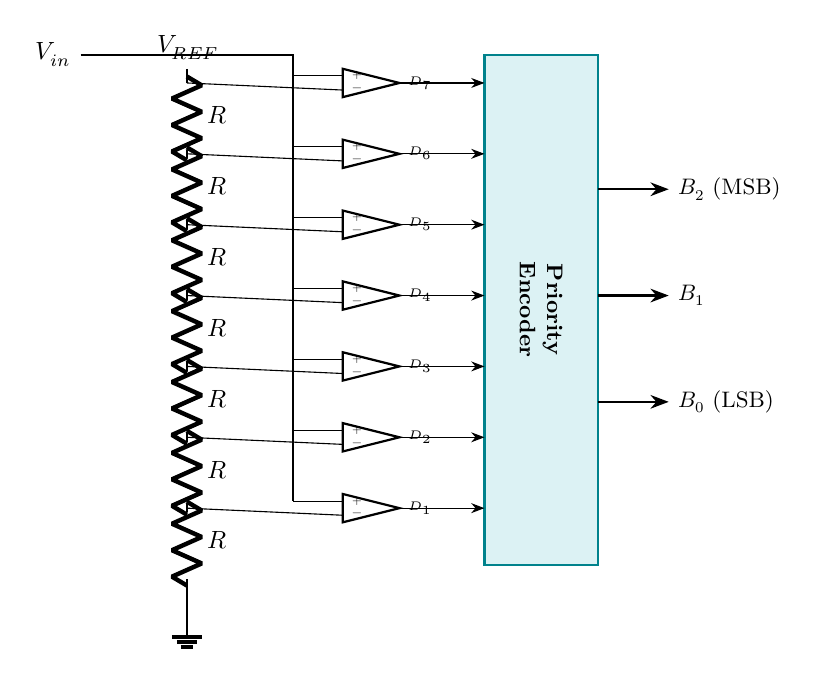
\begin{tikzpicture}[scale=0.9, transform shape]
  % Resistor ladder
  \draw[thick] (0, 3.2) node[above] {$V_{REF}$} -- (0, 3) to[R, l=$R$] (0, 2) to[R, l=$R$] (0, 1) to[R, l=$R$] (0, 0) to[R, l=$R$] (0, -1) to[R, l=$R$] (0, -2) to[R, l=$R$] (0, -3) to[R, l=$R$] (0, -4) -- (0, -4.4) node[ground] {};

  % Comparators
  \foreach \y/\i in {3/7, 2/6, 1/5, 0/4, -1/3, -2/2, -3/1} {
    \draw[thick] (2.2, \y-0.2) -- (2.2, \y+0.2) -- (3.0, \y) -- cycle;
    \node[font=\tiny] at (2.4, \y+0.1) {$+$};
    \node[font=\tiny] at (2.4, \y-0.1) {$-$};
    \node[right, font=\tiny] at (3.0, \y) {$D_{\i}$};
    
    % Connections
    \draw (0, \y) -- (2.2, \y-0.1); % connects to negative
  }

  % Common input line Vin
  \draw[thick] (-1.5, 3.4) node[left] {$V_{in}$} -- (1.5, 3.4) -- (1.5, -2.9);
  \foreach \y in {3, 2, 1, 0, -1, -2, -3} {
    \draw (1.5, \y+0.1) -- (2.2, \y+0.1); % connects to positive
  }

  % Encoder Block
  \draw[thick, fill=hdrteal, draw=myteal] (4.2, -3.8) rectangle (5.8, 3.4);
  \node[rotate=-90, font=\small\bfseries, align=center] at (5.0, -0.2) {Priority\\Encoder};
  
  % Connections from comparators to encoder
  \foreach \y in {3, 2, 1, 0, -1, -2, -3} {
    \draw[-Stealth] (3.0, \y) -- (4.2, \y);
  }

  % Outputs
  \draw[-Stealth, thick] (5.8, 1.5) -- (6.8, 1.5) node[right, font=\small] {$B_2$ (MSB)};
  \draw[-Stealth, thick] (5.8, 0.0) -- (6.8, 0.0) node[right, font=\small] {$B_1$};
  \draw[-Stealth, thick] (5.8, -1.5) -- (6.8, -1.5) node[right, font=\small] {$B_0$ (LSB)};
\end{tikzpicture}
\end{tcolorbox}

\begin{itemize}[leftmargin=*, itemsep=2pt]
  \item \textbf{Working:} The resistor ladder sets $2^N-1$ reference voltages. The comparators simultaneously compare $V_{in}$ to these references, producing a thermometer code. The priority encoder translates this thermometer code to an $N$-bit binary code.
  \item \textbf{Pros:} Conversion finishes in a single clock cycle (highest speed, GHz range).
  \item \textbf{Cons:} Component count grows exponentially ($2^N-1$ comparators). Power and input capacitance grow heavily, limiting resolution to 8 bits.
\end{itemize}

\subsection{2. Successive Approximation Register (SAR) ADC (Moderate Speed/Resolution)}
The SAR ADC utilizes a binary search algorithm to resolve the input voltage bit-by-bit over $N$ clock cycles.
\begin{itemize}[leftmargin=*, itemsep=2pt]
  \item \textbf{Working:} The Sample-and-Hold circuit holds $V_{in}$. The SAR logic sets the MSB of the DAC to 1. The comparator compares $V_{in}$ to $V_{DAC}$. If $V_{in} > V_{DAC}$, the MSB remains 1; otherwise, it is reset to 0. The process repeats for the next bit until all $N$ bits are resolved.
  \item \textbf{Pros:} Low power, minimal analog hardware (only 1 comparator, 1 DAC, and control logic).
  \item \textbf{Cons:} Requires $N$ clock cycles per conversion, limiting speed.
\end{itemize}

\subsection{3. Dual-Slope Integrator ADC (High Accuracy/Low Speed)}
A dual-slope ADC integrates the input voltage for a fixed time $T_1$, then de-integrates using a reference voltage $V_{REF}$ until the integrator output returns to zero.
\begin{itemize}[leftmargin=*, itemsep=2.5pt]
  \item \textbf{Working:} The integrator charges up with current $I_1 = V_{in}/R$ for $2^N$ clock cycles. Then, the input is switched to $-V_{REF}$, discharging the integrator back to 0. A counter measures the discharge time $T_2$.
  \item \textbf{Equation:} The peak integrator voltage is $V_p = \frac{V_{in}}{RC} T_1 = \frac{V_{REF}}{RC} T_2 \Rightarrow V_{in} = V_{REF} \frac{T_2}{T_1}$.
  \item \textbf{Pros:} Outstanding noise rejection (integrates thermal noise out). The accuracy is independent of clock frequency and component values ($R$ and $C$).
  \item \textbf{Cons:} Extremely slow ($2^{N+1}$ clock cycles per sample). Used in digital multimeters.
\end{itemize}

\subsection{4. Pipeline ADC (High Speed, Medium-High Resolution)}
A Pipeline ADC achieves high throughput by processing multiple samples concurrently across a chain of stages. Each stage resolves a coarse set of bits, computes the remaining error (residue), amplifies it by $\times 2$, and passes it to the next stage.

\begin{tcolorbox}[tikzbox, title={Pipeline ADC: 1.5-Bit Stage Architecture}]
\centering
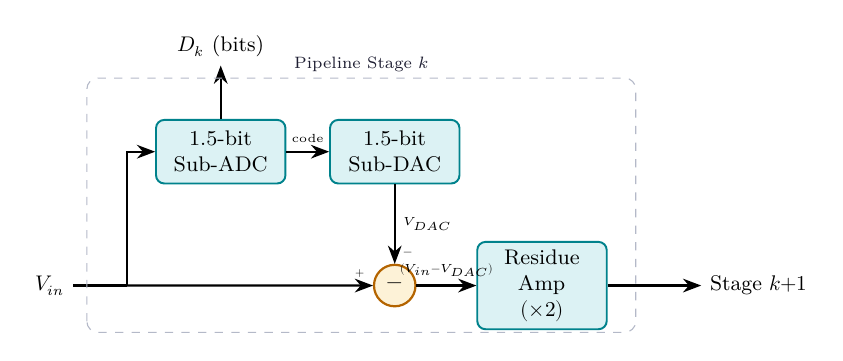
\begin{tikzpicture}[scale=0.85, transform shape]
  % Nodes
  \node[block, text width=1.7cm] (sadc) at (0, 1.2) {1.5-bit\\Sub-ADC};
  \node[block, text width=1.7cm] (sdac) at (2.6, 1.2) {1.5-bit\\Sub-DAC};
  \node[sumjunc] (sub) at (2.6, -0.8) {$-$};
  \node[block, text width=1.7cm] (amp) at (4.8, -0.8) {Residue Amp\\$(\times 2)$};

  % Inputs and Split
  \draw[thick] (-2.2, -0.8) node[left, font=\small]{$V_{in}$} -- (-1.4, -0.8);
  \draw[-Stealth, thick] (-1.4, -0.8) |- (sadc.west);
  \draw[-Stealth, thick] (-1.4, -0.8) -- (sub.west);
  
  \node[above left, font=\tiny] at (sub.west) {$+$};
  \node[above right, font=\tiny] at (sub.north) {$-$};

  % ADC to DAC
  \draw[-Stealth, thick] (sadc.east) -- (sdac.west) node[midway, above, font=\tiny]{code};

  % Digital output
  \draw[-Stealth, thick] (sadc.north) -- ++(0, 0.8) node[above, font=\small]{$D_k$ (bits)};

  % DAC to subtractor
  \draw[-Stealth, thick] (sdac.south) -- (sub.north) node[midway, right, font=\tiny]{$V_{DAC}$};

  % Subtractor to amp
  \draw[-Stealth, thick] (sub.east) -- (amp.west) node[midway, above, font=\tiny]{$(V_{in}{-}V_{DAC})$};

  % Output to next stage
  \draw[-Stealth, thick] (amp.east) -- ++(1.4, 0) node[right, font=\small]{Stage $k{+}1$};

  % Stage bounding box
  \draw[dashed, color=mgframe, rounded corners=4pt] (-2.0, -1.5) rectangle (6.2, 2.3);
  \node[font=\scriptsize\color{mydark}] at (2.1, 2.5) {Pipeline Stage $k$};
\end{tikzpicture}
\end{tcolorbox}

\textbf{Working (1.5-bit/stage):}
\begin{enumerate}[label=\textbf{\arabic*.}, leftmargin=*, itemsep=3pt]
  \item \textbf{Sub-ADC:} A 2-comparator flash resolves the MSBs using three levels ($+1$, $0$, $-1$) compared against $\pm V_{REF}/4$.
  \item \textbf{Sub-DAC:} The coarse code is converted back to an analog level $V_{DAC}$.
  \item \textbf{Residue Amplifier (MDAC):} Computes $V_{res} = 2(V_{in} - V_{DAC})$, scaling the residue to fill the full input range of the next stage.
  \item \textbf{Pipelining:} While Stage 1 processes sample $n+1$, Stage 2 concurrently processes the residue of sample $n$. This gives one output code per clock cycle after an initial latency of $N_{stages}$ cycles.
  \item \textbf{Digital Error Correction:} The 0.5-bit redundancy allows the back-end logic to correct comparator offset errors up to $\pm V_{REF}/4$, relaxing hardware specifications significantly.
\end{enumerate}
\begin{itemize}[leftmargin=*, itemsep=2pt]
  \item \textbf{Pros:} High throughput (10\,Msps--1\,Gsps), excellent resolution (10--14 bits).
  \item \textbf{Cons:} Multi-cycle pipeline latency; MDAC gain accuracy critically limits INL.
\end{itemize}

\subsection{5. Hybrid ADC Structures}
Hybrid ADCs merge two architectures to combine the speed strength of one with the resolution or power efficiency of the other.

\begin{tcolorbox}[defbox, title={\textbf{Common Hybrid ADC Topologies}}]
\begin{itemize}[leftmargin=*, itemsep=4pt, topsep=0pt]
  \item \textbf{Flash-SAR Hybrid:} A coarse Flash ADC resolves the top $M$ bits in a single cycle; a SAR ADC then refines the residue over $N{-}M$ cycles. Reduces comparator count from $2^N - 1$ (full Flash) to $2^M + N - M$, saving power while maintaining near-Flash speed.
  \item \textbf{Pipelined-SAR (SAR-assisted Pipeline):} Each pipeline stage employs a short SAR loop (4--6 bits) instead of the traditional 1.5-bit MDAC. This reduces the total number of stages and relaxes the MDAC gain-bandwidth requirement. Dominant in 10--14-bit, 50--500\,Msps ADCs in modern scaled CMOS nodes.
  \item \textbf{Incremental $\Delta\Sigma$ ADC:} Resets its accumulator after each conversion cycle, combining $\Delta\Sigma$ noise-shaping with discrete Nyquist-rate output. Used in precision multi-channel sensor readout (industrial, medical, weighing systems).
\end{itemize}
\end{tcolorbox}

\subsection{6. Delta-Sigma (\texorpdfstring{$\Delta\Sigma$}{Delta-Sigma}) ADC (Oversampling \& Noise Shaping)}
Delta-Sigma ADCs achieve ultra-high resolution ($16\text{--}24$ bits) by combining \textbf{Oversampling} and \textbf{Noise Shaping}.

\begin{tcolorbox}[tikzbox, title={First-Order Delta-Sigma Modulator Block Diagram}]
\centering
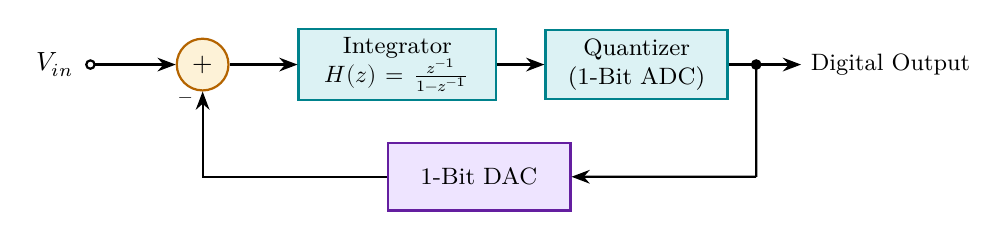
\begin{tikzpicture}[scale=0.95, transform shape]
  % Input
  \node[left] at (-1.6, 0) {$V_{in}$};
  
  % Summer
  \node[draw=myamber, fill=hdramber, circle, minimum size=0.6cm, thick] (sum) at (0, 0) {$+$};
  \draw[-Stealth, thick] (-1.5, 0) to[short, o-] (sum.west);
  
  % Integrator
  \node[draw=myteal, fill=hdrteal, minimum width=1.5cm, minimum height=0.9cm, font=\small, thick, align=center, text width=2.4cm] (int) at (2.6, 0) {Integrator\\$H(z) = \frac{z^{-1}}{1-z^{-1}}$};
  \draw[-Stealth, thick] (sum) -- (int);
  
  % Quantizer (ADC)
  \node[draw=myteal, fill=hdrteal, minimum width=1.4cm, minimum height=0.9cm, font=\small, thick, align=center, text width=2.2cm] (quant) at (5.8, 0) {Quantizer\\(1-Bit ADC)};
  \draw[-Stealth, thick] (int) -- (quant);
  
  % Output
  \draw[-Stealth, thick] (quant) -- (8.0, 0) node[right, font=\small] {Digital Output};
  \draw[thick] (7.4, 0) to[short, *-] (7.4, -1.5);
  
  % Feedback DAC
  \node[draw=mypurple, fill=hdrpurple, minimum width=1.4cm, minimum height=0.9cm, font=\small, thick, align=center, text width=2.2cm] (dac) at (3.7, -1.5) {1-Bit DAC};
  \draw[-Stealth, thick] (7.4, -1.5) -- (dac);
  \draw[-Stealth, thick] (dac) -| (sum) node[left, pos=0.95, font=\scriptsize] {$-$};
\end{tikzpicture}
\end{tcolorbox}

\textbf{Oversampling:} The input is sampled at $f_s \gg 2f_{max}$. The Oversampling Ratio is $\text{OSR} = f_s / (2 f_{max})$. Oversampling spreads the same quantization noise power $\Delta^2/12$ over a wider bandwidth $f_s/2$, reducing the noise spectral density in the signal band.

\textbf{Noise Shaping:} By placing the quantizer inside a feedback loop with an integrator, the transfer function shapes the quantization noise. The output in the Z-domain is:
\[
Y(z) = X(z) z^{-1} + E(z)(1 - z^{-1})
\]
This shows that the input signal $X(z)$ is passed with a simple delay (Signal Transfer Function $\text{STF}(z) = z^{-1}$), while the quantization noise $E(z)$ is high-pass filtered (Noise Transfer Function $\text{NTF}(z) = 1-z^{-1}$). The noise is pushed out of the low-frequency signal band into high frequencies, where it is easily removed by a digital decimation filter.

% ===============================================================================
\section{Digital-to-Analog Converter (DAC) Architectures}
% ===============================================================================

\subsection{1. R-2R Ladder DAC (Compact Layout)}
Unlike binary-weighted resistor DACs (which require huge component ratios like $2^N:1$), the R-2R ladder uses only two resistor values ($R$ and $2R$), making matching very easy.

The output voltage is:
\[
V_{out} = V_{REF} \sum_{i=1}^{N} \frac{b_i}{2^i}
\]
where $b_1$ is the MSB and $b_N$ is the LSB.

\subsection{2. Current-Steering DAC (High Speed)}
Current-steering DACs route currents from matched MOS current sources to the output node based on the digital input code.
\begin{itemize}[leftmargin=*, itemsep=2pt]
  \item \textbf{Working:} An array of current sources (either binary-weighted or thermometer-coded) is connected to differential switches. Thermometer coding is preferred for high resolution because it guarantees monotonicity and minimizes output glitches, though it requires a thermometer decoder.
  \item \textbf{Pros:} Extremely fast (up to GHz range), can drive resistive loads (like $50\,\Omega$ coaxial cables) directly.
\end{itemize}

% ===============================================================================
% QUICK REVISION PAGE
% ===============================================================================
\newpage
\begin{center}
  {\large\bfseries\color{myred} Quick Revision --- Module 3}\\[3pt]
  {\small\color{mydark} Data Converters $|$ PE-EC802A}
\end{center}
\noindent{\color{myred}\rule{\linewidth}{1.2pt}}
\vspace{4pt}

\begin{tcolorbox}[formulabox, title={\textbf{Key Formulas at a Glance}}]
\renewcommand{\arraystretch}{1.35}
\begin{tabularx}{\linewidth}{B{5.0cm} X}
Quantization Error Power & $P_{qn} = \frac{\Delta^2}{12}$ \\[4pt]
Ideal SQNR (dB) & $\text{SQNR} = 6.02 N + 1.76\,$dB \\[4pt]
Oversampling Ratio (OSR) & $\text{OSR} = \frac{f_s}{2 f_{max}}$ \\[4pt]
1st-Order Modulator NTF & $\text{NTF}(z) = 1 - z^{-1}$ \\[4pt]
2nd-Order Modulator NTF & $\text{NTF}(z) = (1 - z^{-1})^2$ \\[4pt]
Flash Comparator Count & $N_{comp} = 2^N - 1$ \\[4pt]
Dual-Slope conversion time & $T_{conv} \approx 2^{N+1} T_{clk}$ \\
\end{tabularx}
\end{tcolorbox}

\begin{tcolorbox}[defbox, title={\textbf{One-Line Definitions}}]
\begin{itemize}[leftmargin=*, itemsep=2pt, topsep=0pt]
  \item \textbf{DNL:} The deviation of an actual step size from the ideal $1\,\text{LSB}$ step width.
  \item \textbf{INL:} The cumulative deviation of the actual transfer curve from the ideal straight line.
  \item \textbf{Oversampling:} Sampling a signal at a rate significantly higher than the Nyquist rate.
  \item \textbf{Noise Shaping:} Pushing quantization noise from the signal band to higher frequencies using feedback loops.
  \item \textbf{Monotonicity:} A converter characteristic where the output always increases or stays constant as input increases.
  \item \textbf{Thermometer Code:} A unary code format representing value $K$ by $K$ consecutive ones (e.g., $3 \rightarrow 0000111$).
  \item \textbf{Missing Codes:} An ADC defect where certain output codes are skipped, caused by $\text{DNL} < -1\,\text{LSB}$.
  \item \textbf{Pipeline ADC:} A high-speed converter using chained 1.5-bit stages with residue amplification, enabling one output per clock cycle.
  \item \textbf{Hybrid ADC:} A converter combining two architectures (e.g., Flash-SAR, Pipelined-SAR) to trade off speed, resolution, and power.
\end{itemize}
\end{tcolorbox}

\begin{tcolorbox}[tikzbox, title={\textbf{ADC Architecture Comparison at a Glance}}]
\centering
\par\noindent
\renewcommand{\arraystretch}{1.25}
\begin{tabularx}{\linewidth}{|B{2.2cm}|Y|Y|Y|Y|}
\hline
\textbf{ADC Type} & \textbf{Speed} & \textbf{Resolution} & \textbf{Power} & \textbf{Application} \\ \hline
\textbf{Flash} & GHz range & $\leq$8 bit & Very High & Oscilloscopes, SerDes \\ \hline
\textbf{SAR} & $<$100\,Msps & 8--18 bit & Very Low & Sensors, IoT, MCUs \\ \hline
\textbf{Dual-Slope} & $<$100 sps & 20+ bit & Low & Multimeters \\ \hline
\textbf{Pipeline} & 10--1000\,Msps & 10--14 bit & Medium & WLAN, Video, RADAR \\ \hline
\textbf{$\Delta\Sigma$} & $<$10\,Msps & 16--24 bit & Medium & Audio, Precision \\ \hline
\textbf{Hybrid} & Varies & Varies & Low--Medium & Imaging, Comm. IC \\ \hline
\end{tabularx}
\end{tcolorbox}

\begin{tcolorbox}[exambox, title={\textbf{Frequently Asked / Viva Questions}}]
\begin{enumerate}[topsep=0pt, label=\textbf{Q\arabic*.}, itemsep=5pt]
  \item \Q{Derive the quantization noise power of an ideal ADC.}
    For a quantization step size $\Delta$, the error $e$ is uniformly distributed between $-\Delta/2$ and $\Delta/2$ with PDF $1/\Delta$. The noise power is the variance: $P_{qn} = \int_{-\Delta/2}^{\Delta/2} e^2 (1/\Delta) de = [e^3/3\Delta]_{-\Delta/2}^{\Delta/2} = \Delta^2/12$.
  \item \Q{What causes missing codes in an ADC, and how is it defined mathematically?}
    Missing codes occur when the transition step width of a digital code is zero or negative. This happens when the Differential Non-Linearity (DNL) at that code is less than or equal to $-1\,\text{LSB}$.
  \item \Q{Explain the trade-offs of Flash ADC architecture.}
    Flash ADC is the fastest architecture because it performs parallel comparisons in one clock cycle. However, it requires $2^N - 1$ comparators. This causes exponential growth in area, power dissipation, and input capacitance, limiting the resolution to 8 bits.
  \item \Q{How does a Delta-Sigma ADC achieve very high resolution?}
    By combining oversampling (which spreads quantization noise over a wider band) and noise shaping (which uses a loop filter to push noise to high frequencies). A digital low-pass decimation filter then filters out the out-of-band noise, leaving a high-resolution signal.
  \item \Q{Why is a dual-slope ADC highly accurate, and where is it used?}
    Its accuracy depends only on the ratio of charging and discharging times ($T_2/T_1$), which is independent of the absolute values of $R$, $C$, and clock frequency. It is used in digital multimeters where accuracy is critical and speed is not.
  \item \Q{Compare SAR and Flash ADCs in terms of speed, area, and power.}
    Flash ADC converts in 1 clock cycle but requires $2^N-1$ comparators (huge area and power). SAR ADC takes $N$ clock cycles but requires only 1 comparator and 1 DAC, resulting in very low power and compact area.
  \item \Q{What is the benefit of the R-2R ladder DAC over a binary-weighted resistor DAC?}
    A binary-weighted resistor DAC requires a very wide range of resistor values ($2^N:1$), which is difficult to match on-chip. The R-2R ladder DAC uses only two resistor values ($R$ and $2R$), ensuring excellent matching and layout compacting.
  \item \Q{Explain the function of the priority encoder in a Flash ADC.}
    The comparators output a thermometer code (e.g. 0000111). The priority encoder identifies the highest active input line and converts that thermometer code into standard binary output (e.g. 011).
  \item \Q{What is the Noise Transfer Function (NTF) of a first-order Delta-Sigma modulator?}
    The NTF is a high-pass filter: $\text{NTF}(z) = 1 - z^{-1}$. In the frequency domain, it is $2 \sin(\omega T_s /2)$, which attenuates noise near DC and amplifies it at high frequencies.
  \item \Q{What is the difference between DNL and INL?}
    DNL is the local step size error from the ideal $1\,\text{LSB}$ step width. INL is the global deviation of the actual transfer function from the ideal straight line, equal to the cumulative sum of the DNL errors.
\end{enumerate}
\end{tcolorbox}

\end{document}
